
\subsection{Mesencephalon}
\label{subsec:Mesencephalon} \index{Mesencephalon}
%%%%%%%%%%%%%%%%%%%%%%%%%%%%%%%%%%%%%%%%%%%%%%%%%%%%%%%%%%%
%%%%%%%%%%%%%%%%%%%%%%%%%%%%%%%%%%%%%%%%%%%%%%%%%%%%%%%%%%%

Im Mesencephalon ist, ähnlich wie bei der Medulla und dem Rückenmark, eine funktionelle Gliederung in die motorische Grundplatte und die sensorische Flügelplatte erkennbar. Dabei sind die motorischen Kerngebiete ventral, bzw. inferior im Tegmentum gelegen. Die sensorischen Kerngebiete liegen dorsal, bzw. superior im Tectum \textsuperscript{\cite[Kap.~6]{trepel2011neuroanatomie}}. Das Mesencephalon umgibt das Aquädukt des Ventrikelsystems.

\subsubsection{Tectum: Vierhügelplatte}
\index{Tectum} \index{Vierhügelplatte}
%%%%%%%%%%%%%%%%%%%%%%%%%%%%%%%%%%%%%%%%%%%%%%%%%%%%%%%%%%%
\label{subsubsec:Tectum}
Das Tectum liegt caudal des diencephalen präoptischen Areals und ist dorsal, bzw. superior im Mesencephalon lokalisiert. Es besteht aus der Vierhügelplatte, auch \textit{Lamina tecti} oder \textit{Lamina quadrigemina} genannt. Diese besteht, wie der Name impliziert, aus vier Schwellungen, den paarigen Colliculi superiores und den ebenfalls paarigen Colliculi inferiores \textsuperscript{\cite[Kap.~6]{trepel2011neuroanatomie}}.\\

\noindent Die geschichteten \textbf{Colliculi superiores}\index{Colliculus! superior} enthalten wichtige Kerngebiete, die an der Entstehung und Steuerung der Augenbewegungen beteiligt sind. Über den Nervus opticus, bzw. Tractus opticus erhalten die oberen Colliculi direkte afferente Informationen von der Retina. Weitere Afferenzen kommen über den Tractus corticospinalis aus der Großhirnrinde, über den Tractus spinotectalis aus dem Rückenmark, sowie aus den Colliculi inferiores. Die efferenten Fasern aus den superioren Colliculi ziehen zu den Hirnnervenkernen (Kap.~\ref{subsec:Myelencephalon}), zur Formatio reticularis (Kap.~\ref{subsec:Hirnstamm}) und ins Rückenmark. Funktionell spielen die Colliculi superiores bei der Entstehung visueller Sakkaden, ruckartigen Bewegungen nach Fixationsphasen, eine wichtige Rolle. Auch beim  Akkommodationsreflex, der automatischen Anpassung der Linsenkrümmung um das Abbild der Außenwelt auf der Retina scharf zu stellen, könnten sie beteiligt sein. Zusammengefasst sind die Colliculi superiores in die Entstehung und Steuerung visueller Reflexe und Augenbewegungen involviert \textsuperscript{\cite[Kap.~6]{trepel2011neuroanatomie}}.\\

\noindent Die \textbf{Colliculi inferiores}\index{Colliculus! inferior} liegen direkt inferior der Colliculi superiores. In ihnen werden fast alle Fasern der Hörbahn verschaltet. Somit stellen sie eine wichtige Station der Hörbahn dar (Kap.~\ref{fig:hoerbahn_pathway}). Die afferenten Fasern treffen über den lateralen Lemniscus ein. Die efferenten Fasern werden über das Brachium colliculi inferioris zum Corpus geniculatum mediale im Thalamus geleitet \textsuperscript{\cite[Kap.~6]{trepel2011neuroanatomie}}.

\begin{figure}[H]
    \centering
    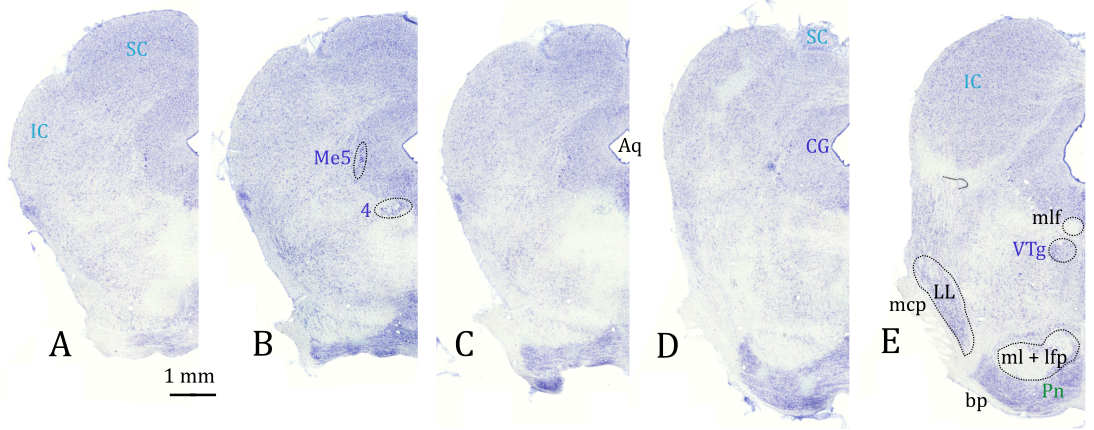
\includegraphics[width=\textwidth]{pictures/Bilder_Jule/Ratte/SC_IC.png}
    \caption[Vierhügelplatte Ratte]{\textbf{Vierhügelplatte Ratte.} Coronalschnitte von caudal nach rostral (A-E: N13-2, N14-1, N14-3, N14-4, N15-1). Teile des Cortex, die über dem Mittelhirn liegen, wurden entfernt. Bereiche des Tectums sind hellblau gekennzeichnet. Dazu gehören der Colliculus inferior (IC) und der Colliculus superior (SC). Bereiche des Tegmentums sind dunkelblau markiert. Dazu gehören das zentrale Höhlengrau (CG), der Nucleus trochlearis (4), die mesencephalen Nuclei des Nervus trigeminus (Me5), so wie der ventrale Nucleus des Tegmentums (VTg). Ebenfalls zu sehen sind das Aquädukt (Aq) des Mesencephalons und die Nuclei pontis (Pn), die dem Metencephalon zuzuordnen sind. Diese metencephalen Strukturen sind grün gekennzeichnet. Weitere Kennzeichnungen: Nuclei des lateralen Lemniscus (LL), medialer Lemniscus (ml), mediales Kleinhirn-Pedunkel (mcp), medialer longitudinaler Fasciculus (mlf), longitudinaler Fasciculus des Pons (lfp), Brachium pontis (bp). \index{Colliculus! superior} \index{Colliculus! inferior}}
    \label{fig:vierhuegelplatte_ratte}
\end{figure}{}

\subsubsection{Tegmentum mesencephali}
\index{Tegmentum! mesencephali}
%%%%%%%%%%%%%%%%%%%%%%%%%%%%%%%%%%%%%%%%%%%%%%%%%%%%%%%%%%%

Der im Mesencephalon lokalisierte Teil des Tegmentums befindet sich inferior des Tectums. Es besitzt hauptsächlich motorische Funktionen. So liegen in ihm wichtige Kerngebiete des (extrapyramidalen) motorischen Systems \textsuperscript{\cite[Kap.~14]{penzlin2005tierphys}}.
Auch die Kerngebiete der Hirnnerven III. (N. oculomotorius) und IV. (N. trochlearis), sowie die motorischen Kerne des Hirnnerven V. (N. trigeminus) sind im mesencephalen Tegmentum lokalisiert \textsuperscript{\cite[Kap.~6]{trepel2011neuroanatomie}}.\\

\noindent Der \textbf{Nucleus ruber}\index{Nucleus! ruber}, ein großer runder Komplex, ist mittig im Tegmentum mesencephali gelegen. Seine rötliche Färbung ist auf einen hohen Eisengehalt zurückzuführen. Afferenzen erhält der Nucleus ruber aus Cortex und Cerebellum. Efferenzen aus dem N. ruber ziehen über den Tractus rubrospinalis\index{Tractus! rubrospinalis} zum Rückenmark, über den Tractus rubroreticularis\index{Tractus! rubroreticularis} in die Formatio reticularis (Kap.~\ref{subsec:Hirnstamm}) und über den Tractus rubroolivaris\index{Tractus! rubroolivaris} in die Olive. Funktionell dient der Nucleus ruber als wichtige Schaltstelle des motorischen Systems (Kap.~\ref{sec:Motorik}). Durch seine Projektionen ins Rückenmark ist er Teil des extrapyramidalmotorischen Systems \textsuperscript{\cite[Kap.~6]{trepel2011neuroanatomie}}.\\

\begin{figure}[H]
    \centering
    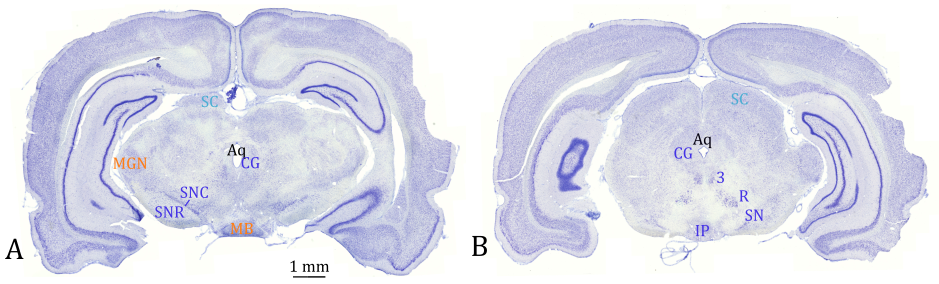
\includegraphics[width=\textwidth]{pictures/Bilder_Jule/Ratte/tegmentum_mesenc.png}
    \caption[Tegmentum Ratte]{\textbf{Tegmentum Ratte.} Coronalschnitte durch das Tegmentum mesencephali. Die Schnitte sind von rostral nach caudal angeordnet (A:~N18-4, B:~N16-2). Teilgebiete des Tegmentums sind dunkelblau gekennzeichnet. Dazu gehören das zentrale Höhlengrau (CG), das das Aquädukt (Aq) umgibt, die Substantia nigra (SN), die in die Pars compacta (SNP) und Pars reticulata (SNR) unterteilt ist, sowie der Nucleus ruber (R), die Nuclei des Nervus oculomotorius (3) und der unpaare Nucleus interpeduncularis (IP). Teilgebiete des Tectums, wie die Colliculi superiores (SC) sind hellblau markiert. Rostral sind zudem Teile des Diencephalons (orange), wie der Nucleus geniculatum mediale (MGN) und der Mammillarkörper (MB) zu sehen.}
    \label{fig:tegmentum_mesenc}
\end{figure}{}

\noindent Auch die \textbf{Substantia nigra}\index{Substantia nigra}, die funktionell den Basalganglia (Kap.~\ref{subsec:basalganglien}) unterzuordnen ist, ist im Tegmentum lokalisiert. Die dunkle Farbe des Kerngebiets ist durch einen hohen Melanin-Gehalt zu erklären. Generell kann die Substantia nigra in die S.n. \textbf{pars compacta} und die S.n. \textbf{pars reticularis} unterteilt werden. Beiden sind unterschiedliche Faserverbindungen und Funktionen zuzuordnen \textsuperscript{\cite[Kap.~6]{trepel2011neuroanatomie}}. 
Ausgehend von der Substantia nigra pars compacta erstrecken sich Neurone, die Dopamin enthalten, bis hin zu einer Struktur, die \textbf{Area tegmentalis ventralis (VTA)}\index{Area tegmentalis ventralis} genannt wird. Die dopaminergen Neurone der VTA sind elementarer Bestandteil des dopaminergen Systems (Kap.~\ref{dopaminerges_system}).
Der Großteil der Projektionen aus der pars compacta enden im Striatum. \textsuperscript{\cite[Kap.~9]{crossman2014neuroanatomy}}. Funktionell ist sie in die Kontrolle und Modulation von Bewegungsimpulsen und Bewegungsabläufen involviert. Die Degeneration dopaminerger Neurone der Substantia nigra führt zum Krankheitsbild \textbf{Morbus Parkinson}\index{Morbus Parkinson}. Folgen sind Zittern (Tremor) in Ruhephasen, erhöhter Muskeltonus in Verbindung mit steifer Muskulatur (Rigor), sowie Bewegungsarmut (Akinese) \textsuperscript{\cite[Kap.~6]{trepel2011neuroanatomie}}. \\

\noindent Das \textbf{zentrale Höhlengrau}\index{zentrales Höhlengrau}, auch periaquäduktales Grau oder \textit{Griseum centrale}, ist ein dunkleres, Birnen-förmiges  Kerngebiet, das medial im Mesencephalon liegt. Es umschließt das Aquädukt ähnlich wie die graue Substanz des Rückenmarks den Zentralkanal. Etwa auf gleicher Höhe des superioren und inferioren Colliculus liegen die Nuclei des N. trochlearis und des N. oculomotorius, die äußere Augenmuskulatur innervieren und somit die Augenbewegungen steuern \textsuperscript{\cite[Kap.~9]{crossman2014neuroanatomy}}. Des Weiteren ist das periaquäduktale Grau Teil des Schmerz-Systems (Kap.~\ref{subsubsec:Schmerzsinn}) \textsuperscript{\cite[Kap.~25]{paxinos2014rat}}
